\section{When MMIO Direct Push Hurts Neighbors}
\label{sec:host_contention}

We begin by examining how sustained posted MMIO writes affect co-located applications sharing the same host socket. On Socket~1, we pin co-located victim workloads to fixed physical cores (\texttt{cpu40..45} for 6-core STREAM Triad~\cite{mccalpin1995stream} and Copy; \texttt{cpu40} for 16\,MiB L3 and 256\,MiB DRAM pointer chasing, with SMT siblings \texttt{cpu104..109} kept strictly idle) and run MMIO direct-push aggressors on disjoint physical cores across two targets: off-chip CN106 \texttt{BAR4} (\texttt{IIO1}, 516 runs) and on-die Intel DSA \texttt{wq2.0} (\texttt{IIO0}, 369 + 381 runs).

\begin{figure*}[t]
  \centering
  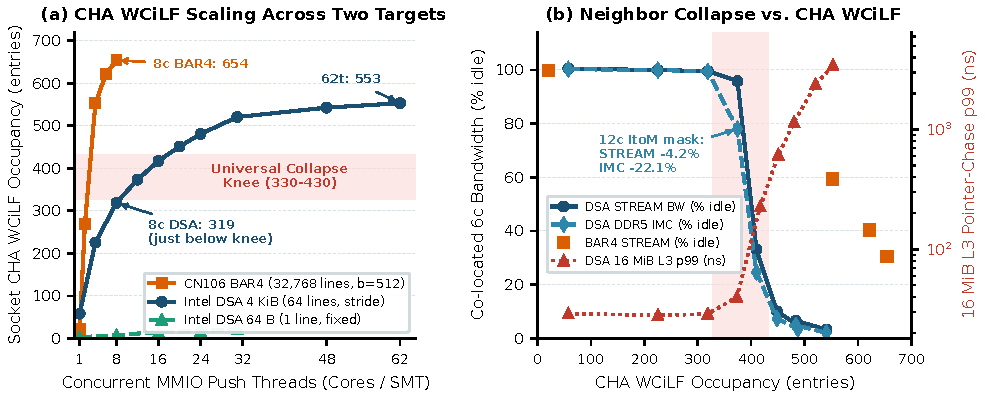
\includegraphics[width=\textwidth]{figures/fig1_host_tor_collapse.pdf}
  \caption{The universal host \texttt{CHA TOR} collapse law across two independent hardware targets. (a)~Socket-wide \texttt{CHA WCiLF} occupancy scales steeply with thread count on both CN106 \texttt{BAR4} (32,768 lines) and the 4\,KiB (64-line) Intel DSA portal, whereas single-line \texttt{noop-fixed} stays capped at $\le$\,21 entries. (b)~Across both targets, crossing the 330--430-entry \texttt{WCiLF} cliff collapses co-located 6-core STREAM Triad bandwidth (up to $-$96.7\%) and spikes 16\,MiB L3 \texttt{p99} latency (up to 116$\times$). At 12-core DSA, physical DDR5 IMC bandwidth already drops $-$22.1\% while Golden Cove's adaptive \texttt{RFO}\,$\to$\,\texttt{ItoM} masks logical STREAM to $-$4.2\%.}
  \label{fig:tor_collapse}
\end{figure*}

\subsection{The Steady-State Dividend vs. Wide-BAR Collapse}
\label{sec:host_bar4}

When a single host core pushes 64\,B \texttt{MOVDIR64B} writes to CN106 \texttt{BAR4} across 50--175\,Mpps (3.2--11.2\,GB/s payload), the isolation promise holds almost completely (\autoref{tab:host_tor}). At 1-core maximum rate (175.3\,Mpps, \texttt{b\,=\,512} \texttt{SFENCE} cadence), socket-wide \texttt{CHA} occupancy stays at 21.1 entries (\texttt{IRP1\,=\,4.15}, \texttt{M2PCIe1} non-empty duty 8.4\%). Co-located 6-core STREAM Triad remains at 49.62\,GB/s vs. 49.76\,GB/s idle ($-$0.3\%), 16\,MiB L3 \texttt{p99} stays at 29.25\,ns vs. 29.75\,ns idle, and 256\,MiB DRAM pointer-chase \texttt{p99} stays at 135.0\,ns vs. 135.0\,ns idle. In contrast, sustaining 160\,Mpps through a traditional host-memory ring pulled by CN106's DMA engine (\texttt{DPI}) directly pollutes L3 or competes for the two DDR5 channels: a 16\,MiB host ring cuts 6-core STREAM Triad by $-$9.9\% (44.86\,GB/s), a 1-core 256\,MiB ring cuts it by $-$20.6\% (39.50\,GB/s), and a 4-core 256\,MiB ring cuts it by $-$41.0\% (29.38\,GB/s) while raising DRAM latency by 6.8\%--26.2\%.

Adding unpaced host push cores on \texttt{BAR4}, however, flips this isolation into catastrophic collapse. Because PCIe Gen5\,$\times$4 caps outbound posted writes at 175.5\,Mpps, two cores already saturate \texttt{IRP1} (7.47 entries) and \texttt{M2PCIe1} (90.5\% busy), pushing \texttt{CHA TOR} occupancy to 269.2 entries---still just below the cliff, so STREAM Triad holds at 49.58\,GB/s. At 4, 6, and 8 unpaced cores (\texttt{b\,=\,512}), posted backpressure overflows \texttt{M2PCIe1} (96.8\%--98.8\% busy) into the 32 \texttt{CHA} slices: \texttt{CHA TOR} surges to 552.8, 621.7, and 654.1 entries (with the hottest slice reaching 21.0 entries). Co-located 6-core STREAM Triad collapses by $-$40.6\% (29.54\,GB/s at 4c), $-$59.6\% (20.08\,GB/s at 6c), and $-$69.5\% (15.17\,GB/s at 8c), while 16\,MiB L3 \texttt{p99} balloons 20.2$\times$ from 29.75\,ns to 601.25\,ns and 256\,MiB DRAM \texttt{p99} jumps 8.1$\times$ from 135\,ns to 1,091\,ns. Meanwhile, the 8-core \texttt{l1-spin} control yields 49.69\,GB/s and 29.5\,ns, ruling out turbo down-clocking.

\subsection{Disproving Two Myths on Intel DSA's \texorpdfstring{4\,KiB}{4 KiB} Portal}
\label{sec:host_dsa}

Could a well-engineered NIC portal avoid this cliff either by (1)~dropping overflow writes in hardware instead of stalling PCIe flow control, or (2)~restricting the portal window to a single 4\,KiB page (64 cache lines) rather than a 32,768-line \texttt{BAR4}? Intel DSA \texttt{wq2.0} on \texttt{IIO0} implements \emph{both} properties in real silicon.

\para{Myth 1: Hardware descriptor dropping prevents host backpressure.}
When 8 cores blast 64\,B \texttt{MEMMOVE} descriptors across DSA's 4\,KiB portal (142.2\,Mpps), the 128-entry \texttt{DWQ} overflows and hardware discards 94.6\% of descriptors via \texttt{SWERROR}. Yet co-located 6-core STREAM Triad drops by only $-$2.2\% (48.92 vs. 50.00\,GB/s), and 16\,MiB L3 \texttt{p99} stays unchanged (29.0\,ns). Crucially, hardware counters prove this is \emph{not} because dropping avoids backpressure: \texttt{IRP0} is pinned at 7.71 entries, \texttt{M2PCIe0} is 99.9\% busy, and \texttt{CHA WCiLF} residency stretches to 2.16--2.23\,\textmu s. Rather, at 8 cores the 64-line portal accidentally caps socket-wide \texttt{WCiLF} at 309.1--318.8 entries---just shy of the 330-entry cliff!

The moment DSA simultaneously executes active 64\,KiB \texttt{MEMMOVE} transfers over the same \texttt{IIO0} stack, total \texttt{CHA TOR} occupancy (portal \texttt{WCiLF} + inbound DMA) jumps to 467--593 entries (472 under DRAM chase). Even with 22--25\,GB/s of unused DDR5 headroom (\texttt{IMC} drops from 63.7 down to 38.2--41.5\,GB/s), co-located 6-core STREAM Triad plunges by $-$43.5\% to $-$47.7\% (26.14--28.24\,GB/s), L3 \texttt{p99} rises to 117.3\,ns, and the portal flood simultaneously slashes DSA's own 64\,KiB DMA throughput by 77\% (from 61.1 down to 13.9--14.1\,GB/s under \texttt{IIO0} 1.00\,GHz cycle conservation).

\para{Myth 2: A single 4\,KiB (64-line) portal is inherently safe.}
To test whether 8-core safety on pure \texttt{NOOP} traffic (0 DMA, \texttt{dwq\_full\,=\,0}) was a structural 64-line cap or merely a core-count coincidence, we scaled pure \texttt{noop-stride} across 1--32 physical cores and up to 62--64 SMT threads on Socket~1 (\autoref{fig:tor_collapse}a--\ref{fig:tor_collapse}b, \autoref{tab:host_tor}). The 64-line page offers \emph{no} global cap:
\begin{itemize}
  \item \textbf{12 cores enter the cliff (\texttt{WCiLF\,=\,373.6}):} Logical 6-core STREAM Triad appears to dip only $-$4.2\% (50.20\,$\to$\,48.09\,GB/s), yet physical DDR5 \texttt{IMC} bandwidth has already fallen $-$22.1\% (58.74\,$\to$\,45.77\,GB/s) and \texttt{IMC RPQ} occupancy is cut nearly in half (46.2\,$\to$\,23.9). The mismatch comes from Golden Cove's adaptive write-allocate policy~\cite{mccalpin2023spr}: under rising \texttt{TOR} latency, the core shifts STREAM store misses from Read-For-Ownership (\texttt{RFO}, 1 read + 1 write = 3 DRAM accesses per Triad iteration) to \texttt{ItoM} (0 read + 1 write = 2 DRAM accesses), temporarily masking a 22\% memory-system collapse as a 4\% application dip.
  \item \textbf{16 cores cross the cliff (\texttt{WCiLF\,=\,418.5}):} The hottest \texttt{CHA} slice hits its effective ceiling (22.0 entries). Co-located 6-core STREAM Triad plunges $-$67.0\% (16.57\,GB/s, physical \texttt{IMC} 14.47\,GB/s), and 16\,MiB L3 \texttt{p99} spikes 7.7$\times$ (29.5\,$\to$\,227.25\,ns).
  \item \textbf{24--31 cores and 48--62 SMT threads paralyze the socket:} \texttt{WCiLF} reaches 477.5--553.2 entries (hottest slice pinned at 22.9--23.0). Co-located STREAM Triad collapses by $-$95.1\% to $-$96.7\% (2.45\,$\to$\,1.64\,GB/s; \texttt{IMC\,=\,1.23--2.01\,GB/s}), and 16\,MiB L3 \texttt{p99} explodes 39$\times$--116$\times$ (1,152--3,424\,ns)---with zero DMA and zero dropped descriptors.
\end{itemize}

\begin{table}[t]
  \centering
  \scriptsize
  \setlength{\tabcolsep}{2.2pt}
  \begin{tabular}{@{}lrrrrr@{}}
    \toprule
    \textbf{Target \& Workload} & \textbf{Mpps} & \textbf{CHA} & \textbf{Max} & \textbf{STREAM} & \textbf{L3 p99} \\
    \midrule
    Idle (BAR4 / DSA) & 0.0 & 1.8 & 0.1 & 49.8 / 50.2 & 29.5\,ns \\
    BAR4 1c max (\texttt{b=512}) & 175.3 & 21.1 & 0.7 & 49.6 ($-$0.3\%) & 29.3\,ns \\
    BAR4 4c max (\texttt{b=512}) & 175.4 & 552.8 & 17.5 & 29.5 ($-$40.6\%) & 221.8\,ns \\
    BAR4 8c max (\texttt{b=512}) & 175.5 & 654.1 & 21.0 & 15.2 ($-$69.5\%) & 601.3\,ns \\
    BAR4 8c paced (\texttt{165M,b128}) & 165.1 & 114.4 & 3.7 & \textbf{49.8 (+0.0\%)} & \textbf{29.3\,ns} \\
    Host DMA 16M / 256M 4c & 160.1 & 11--50 & 1.6 & 44.9 / 29.4 & 29.3\,ns \\
    \midrule
    DSA 8c \texttt{stride} (4\,KiB) & 143.1 & 318.6 & 12.8 & 50.0 ($-$0.5\%) & 29.0\,ns \\
    DSA 12c \texttt{stride} (4\,KiB) & 143.1 & 373.6 & 18.5 & 48.1 ($-$4.2\%)$^\dagger$ & 39.8\,ns \\
    DSA 16c \texttt{stride} (4\,KiB) & 143.2 & 418.5 & 22.0 & 16.6 ($-$67.0\%) & 227.3\,ns \\
    DSA 24c \texttt{stride} (4\,KiB) & 144.0 & 477.5 & 22.9 & 2.45 ($-$95.1\%) & 1,152\,ns \\
    DSA 31c / 62t \texttt{stride} & 146.0 & 521--553 & 23.0 & 1.64 ($-$96.7\%) & 3,424\,ns \\
    DSA 24c / 31c \texttt{fixed} (64\,B) & 137.0 & 16.8--21.9 & 20.3 & 59.9 (+19.3\%) & 38.3\,ns \\
    DSA 8c \texttt{64K DMA+stride} & 116.8 & 589.7 & --- & 28.2 ($-$43.5\%) & 117.3\,ns \\
    \bottomrule
  \end{tabular}
  \caption{Summary of host-side neighbor interference across CN106 \texttt{BAR4} and Intel DSA (medians across $n\,=\,3$, 100\% non-multiplexed PMU). STREAM is 6-core Triad (GB/s); CHA is socket-wide occupancy (isolated \texttt{WCiLF} for DSA scaling, total \texttt{TOR} for BAR4 and mixed DMA). $^\dagger$At 12c DSA, physical DDR5 IMC already falls $-$22.1\% (58.74\,$\to$\,45.77\,GB/s), masked by \texttt{ItoM}.}
  \label{tab:host_tor}
\end{table}

\subsection{The Unified Physical Law and Concurrency Bound}
\label{sec:host_law}

Comparing \texttt{noop-stride} (64 lines), \texttt{noop-fixed} (1 line), and \texttt{BAR4} (32,768 lines) isolates the exact microarchitectural mechanism. First, \texttt{noop-fixed} at 31 physical cores injects 137.0\,Mpps of \texttt{NCB} mesh traffic---within 5\% of \texttt{noop-stride}'s 144.5\,Mpps---yet keeps socket-wide \texttt{WCiLF} at 21.9 entries (confined to a single \texttt{CHA} slice) and leaves 6-core STREAM Triad completely unharmed (59.87\,GB/s at 24c, even rising due to \texttt{ItoM}) and L3 \texttt{p99} at 38.3\,ns. This proves the collapse is \emph{not} 2D mesh data-ring bandwidth contention, nor is it LLC capacity eviction (SPR's non-inclusive L3 bypasses fills for 99.5\%--99.85\% of \texttt{WCiLF} writes).

Instead, the collapse is pure \textbf{\texttt{CHA TOR} slot exhaustion}. Every \texttt{CHA} slice has a finite pool of \texttt{TOR} entries shared between coherent memory requests and posted \texttt{WCiLF} writes; once the hottest slices approach $\sim$22--23 occupied entries (corresponding to 330--430 socket-wide \texttt{WCiLF} entries under uniform or 64-line hashing), co-located loads and stores stall waiting for \texttt{TOR} allocation, collapsing memory-level parallelism (\texttt{IMC RPQ} falls from 46.2 to 0.2--3.8).

Second, why did \texttt{noop-fixed} scale to 16.8--20.6 entries at 24--32 cores, and why did \texttt{16c\,$\times$\,2} SMT (32 threads) exceed 16 physical cores (17.25 > 16 entries on a single line, and 480.2 vs. 418.5 on 64 lines)? Because x86 serializes same-line posted writes inside each core's write-combining/fill buffers at the granularity of a \textbf{\texttt{(Physical Core WCB, 64\,B line)} pair}: each active thread can hold at most one outstanding \texttt{WCiLF} per distinct destination cache line, different physical cores can concurrently queue independent \texttt{WCiLF} transactions to the \emph{same} 64\,B line, and SMT siblings on the same physical core partially coalesce in the shared WCB when wrapping onto identical lines (verified directly in \S\ref{sec:eval_disjoint}). Consequently, when $N$ active threads touch $K_i$ non-overlapping MMIO cache lines under downstream backpressure, socket-wide \texttt{CHA WCiLF} occupancy scales linearly with the active line budget $\sum_{i=1}^{N} K_i$. Leaving headroom for coherent traffic, background non-temporal stores (\eg{} AVX2 \texttt{VMOVNTPD}), and hottest-slice hashing skew, an unpaced MMIO portal must satisfy:
\begin{equation}
  \sum_{i=1}^{N} K_i \;<\; 200.
  \label{eq:concurrency}
\end{equation}
For a shared 4\,KiB page ($K_i\,=\,64$), $8 \times 64 = 512$ is already damped by per-core LFB limits to 318.6 entries (just below 330), whereas $12 \times 64 = 768$ pushes \texttt{WCiLF} to 373.6 and $16 \times 64 = 1024$ breaks the socket wide open.
